\documentclass[border=3pt,tikz]{standalone}
% Shared look for every TikZ figure in these notes.
% Included by each standalone figure file; also keeps the figures consistent
% with the colours used in the PDF and on the website.

\usepackage{tikz}
\usepackage{pgfplots}
\pgfplotsset{compat=1.18}
\usetikzlibrary{arrows.meta, decorations.markings, decorations.pathmorphing,
                patterns, calc, positioning}
\usepackage{amsmath}

% Series colours are the three validated categorical slots also used by the
% interactive widgets, so a path drawn in the printed notes and the same path on
% the website are the same colour. They clear the colour-vision-deficiency and
% contrast checks as a set; every path is direct-labelled as well, so colour is
% never the only thing carrying identity.
\definecolor{duPurple}{HTML}{68246D}
\definecolor{duBlue}{HTML}{2A78D6}
\definecolor{duRed}{HTML}{EB6834}
\definecolor{duGreen}{HTML}{1BAF7A}
\definecolor{duGrey}{HTML}{6B6B6B}

\tikzset{
  axisline/.style   = {-{Stealth[length=3mm]}, line width=0.7pt, black},
  path1/.style      = {duBlue,   line width=1.1pt},
  path2/.style      = {duRed,    line width=1.1pt},
  path3/.style      = {duGreen,  line width=1.1pt},
  statedot/.style   = {circle, fill=black, inner sep=1.4pt},
  arrowhead/.style  = {decoration={markings,
                        mark=at position #1 with {\arrow{Stealth[length=2.6mm]}}},
                       postaction={decorate}},
  lbl/.style        = {font=\small},
  slbl/.style       = {font=\footnotesize, duGrey},
  workfill/.style   = {duPurple, opacity=0.16},
}

% Corollary 2 proof: an imaginary engine I (eta_I > eta_R) drives a reversible
% engine R run backwards; both exchange the same |Q_H| with the hot reservoir
\begin{document}
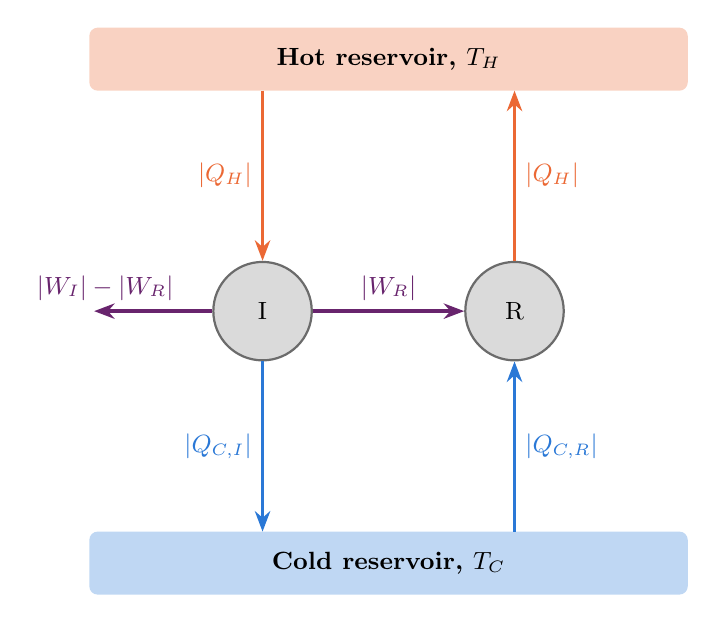
\begin{tikzpicture}[x=1cm,y=1cm,
    res/.style={draw=none, rounded corners=3pt, minimum width=7.6cm, minimum height=0.8cm, font=\small\bfseries},
    eng/.style={circle, draw=duGrey, fill=duGrey!25, line width=0.8pt, minimum size=1.25cm, font=\small},
    flow/.style={-{Stealth[length=2.6mm]}, line width=1.2pt}]
  \node[res, fill=duRed!30] (hot) at (0,3.2) {Hot reservoir, $T_H$};
  \node[res, fill=duBlue!30] (cold) at (0,-3.2) {Cold reservoir, $T_C$};
  \node[eng] (I) at (-1.6,0) {I};
  \node[eng] (R) at (1.6,0) {R};
  % imaginary engine, forwards
  \draw[flow, duRed]  (-1.6,2.8) -- (I.north) node[midway, left, lbl] {$|Q_H|$};
  \draw[flow, duBlue] (I.south) -- (-1.6,-2.8) node[midway, left, lbl] {$|Q_{C,I}|$};
  % reversible engine, backwards (heat pump)
  \draw[flow, duBlue] (1.6,-2.8) -- (R.south) node[midway, right, lbl] {$|Q_{C,R}|$};
  \draw[flow, duRed]  (R.north) -- (1.6,2.8) node[midway, right, lbl] {$|Q_H|$};
  % work: part of W_I drives R, the rest is left over
  \draw[flow, duPurple] (I.east) -- (R.west) node[midway, above, lbl] {$|W_R|$};
  \draw[flow, duPurple] (I.west) -- ++(-1.5,0) node[above, lbl, xshift=4pt] {$|W_I| - |W_R|$};
\end{tikzpicture}
\end{document}
